\documentclass[tikz]{standalone}

\usepackage[T2A]{fontenc}
\usepackage[utf8x]{inputenc}
\usepackage{amsmath,amssymb}
\usepackage{cmap,pgfplots,pgfplotstable}
\pgfplotsset{compat=newest}


\begin{document}
	% \pgfplotstableread{data.tsv}\mytable 
	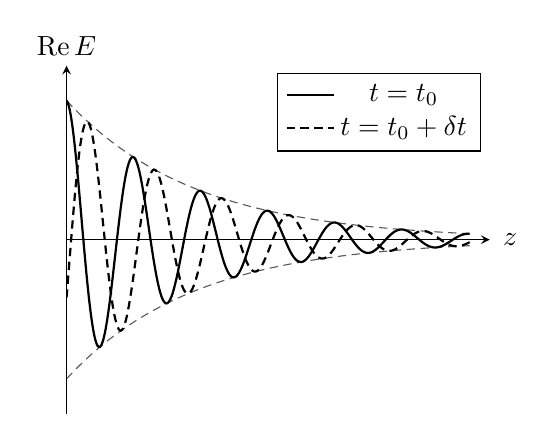
\begin{tikzpicture}
		\begin{axis}[
			% width=7cm,
			height=6 cm,
			% enlargelimits = true,
			% legend pos= south east,
			% legend pos=outer north east,
			ymax = 1.25,
			ymin = -1.25,
			% xmin = 0,
			xmax = 2.1*pi,
			% scale=1,
			ylabel={$\mathrm{Re}\,E$}, 			% подпись оси Y
			xlabel={$z$}, 			% подпись оси X
			% xticklabels={},
			% yticklabels={},
			xtick=\empty,
			ytick=\empty,
			%major grid style={
				%	line width=0.5pt, 	% толщина основных линий сетки
				%	draw=black!50 		% цвет основных линий сетки: 50% черного (80% белого) 
				%},
			minor grid style={
				line width=0.5pt, 	% толщина промежуточных линий сетки
				draw=black!20		% цвет промежуточных линий сетки
			},
			%minor tick num=1,		% количество промежуточных линий между основными
			ticklabel style={
				% scale=0.1			% уменьшим размер подписей меток на осях
			},    
			%xticklabel style={above, yshift=0.25em},
			%yticklabel style={right},
			axis lines=middle, 		% выравнивание оси y:  middle (в нуле)|left|right
			%enlargelimits=true,
			%xtick distance=0.5,		% расстояние между метками по оси X
			%ytick distance=0.5,		% расстояние между метками по оси Y
			% unit vector ratio = 1 1,% масштаб 1:1 осей X и Y
			% clip=false,
			% ymax= 1.5,
			x label style={
				at={(current axis.right of origin)}, 
				xshift=1.7ex, anchor=center
			},
			% extra x ticks={1},	% положение дополнительных тиков
			% extra x tick labels={	% их подписи
				% {$\omega_{cr_{n}}$}
				% }, 		
			y label style={
				% at={(axis description cs:0.01,1.07)},
				yshift=0.7em,
				anchor=center,		% расПоложение метКи ровно в точКе (0,1.1)
				black				% цвет метКи
			},		
			]
			
			\addplot[thick,domain={0:2*pi},samples=350] {exp(-x/2)*cos(deg(x*6))};
			\addlegendentry{$t=t_0$}
			\addplot[thick,densely dashed,domain={0:2*pi},samples=350] {exp(-x/2)*cos(deg(x*6-2))};
			\addlegendentry{$t=t_0+\delta t$}
			\addplot[thin,densely dashed,opacity=0.65,domain={0:2*pi},samples=350] {exp(-x/2)};
			\addplot[thin,densely dashed,opacity=0.65,domain={0:2*pi},samples=350] {-exp(-x/2)};
			
		\end{axis}
	\end{tikzpicture}	
\end{document}